\section{Relative tropical \texorpdfstring{$2$}{2}-cycles}\label{sec:cycles}


This section proves Theorem~\ref{thm:real}: on the base $B=B'_\sigma$ every balanced network is the boundary network
of a relative tropical $2$-cycle, and the node coefficients of balanced networks form exactly the lattice $K$ of
relations among the circuits. The proof is combinatorial topology of the pair $(B,\Gamma)$, a three-sphere and a
graph in it, with the coefficients of Definition~\ref{def:relcycle}. It has two parts.

The \emph{boundary level}, $\rho(\cyBal)=K$ (Section~\ref{ssec:cycles-bdry}), is a statement about flows. A balanced
network splits into one integral $1$-chain for each edge $\varepsilon$ of the subdivision $\Sigma'$ of the two-skeleton
of $\Delta$, supported on the legs whose lower support is $\varepsilon$. The balance conditions at the negative vertices
and nodes say that these $1$-chains assemble into a cellular $1$-chain on $\partial\Delta$, the node coefficients are
read off from its boundary, and $H_1(\partial\Delta;\Z)=0$ produces a balanced network for every $k\in K$.

The \emph{filling}, $\partial Z(\mathfrak K_0)=\cyBal$ (Section~\ref{ssec:filling}), moves a balanced network, by
$2$-chains supported in discs transverse to the cells of $B$, to a $1$-cycle in $B\setminus\Gamma$ with coefficients in
the local system $\Lambda$. The class of that cycle is computed from the cover of $B\setminus\Gamma$ by the open facets
and the vertex regions of $B$, and it lies in the span of the meridians of $\Gamma$ (Lemma~\ref{lem:complement}). The
proof of that lemma has two parts. A Mayer--Vietoris argument over a regular neighbourhood of $\Gamma$, whose homology
relative to its frontier is computed in Section~\ref{ssec:normal}, shows that meridians generate $H_1(B\setminus\Gamma;\Z)$.
A computation on the boundary spheres of the facets of $B$, which uses the dual-pair cells of $B$, the connectedness of
the links of vertices in the triangulated faces of $\Delta^\circ$, $H^1(S^2)=0$, and the fact that the vertices of every
simplex of the unimodular triangulation $\mathcal T$ are part of a basis of $M$, then passes from constant coefficients to
the coefficients $\Lambda$. A meridian with an invariant coefficient bounds a disc that crosses $\Gamma$ once.

Section~\ref{ssec:cbm} shows that the tropical $2$-cycles of Casta\~no-Bernard and Matessi \cite[Def.~7.2]{CBM},
triangulated, are relative tropical $2$-cycles with the same node coefficients. Section~\ref{ssec:normal} computes the
homology of a regular neighbourhood of $\Gamma$ with coefficients in $\iota_*\Lambda$ and deduces a normal form of
relative tropical $2$-cycles near $\Gamma$, which the lift of Section~\ref{sec:lift} uses. Throughout, $\Delta$ is
admissible with a profile $\sigma$ satisfying~\ref{hyp:P}, and $(\mathcal T,\check h)$ is fixed as in
Section~\ref{ssec:tropical}; all homology is integral unless coefficients are named.

\subsection{The coefficient system}\label{ssec:coef}

\emph{The dual-pair cells.} We use the cell decomposition of $B$ by dual pairs of Section~\ref{sec:dualpair}. For a
simplex $\tau$ of $\mathcal T$ and a cell $\omega$ of $\Sigma'$ put
\begin{gather*}
\tau^\vee=\{n\in\Delta:\langle u,n\rangle=-1\text{ for all vertices $u$ of $\tau$}\},\\
\omega^\vee=\{m\in\Delta^\circ:\langle m,n\rangle=-1\text{ for all vertices $n$ of $\omega$}\};
\end{gather*}
$\tau^\vee$ is the face of $\Delta$ dual to the smallest face of $\Delta^\circ$ containing $\tau$, and likewise for $\omega^\vee$.
We write $u^\vee$ for $\{u\}^\vee$, and $\cylin(\omega)\subset N_\R$ for the linear span of the differences of points of
$\omega$, so that $\cylin(\omega)\cap N$ is the lattice of integral vectors parallel to $\omega$. A \emph{dual pair} is a pair
$(\tau,\omega)$ with $\omega\subseteq\tau^\vee$, equivalently $\tau\subseteq\omega^\vee$, that is, $\langle u,n\rangle=-1$ for
every vertex $u$ of $\tau$ and every vertex $n$ of $\omega$ (Definition~\ref{def:DP}). For
a cell $c$ of $\mathscr P$ let $\omega(c)\in\Sigma'$ be its lower support and $\tau(c)\in\mathcal T$ its face label, so that
$F_{\tau(c)}$ is the smallest face of $\nabla^{\check h}$ containing $c$. For a dual pair $(\tau,\omega)$ let
$C(\tau,\omega)\subset B$ be the union of the open simplices of the barycentric subdivision $\mathfrak K_0$ of $\mathscr P$
whose chains $c_0\subsetneq\dots\subsetneq c_k$ have $\tau(c_k)=\tau$ and $\omega(c_0)=\omega$; this is the cell
$C_X(\tau,\omega)$ of Definition~\ref{def:strata}. The following facts are
Propositions~\ref{prop:L1}(2),(4),(5) and~\ref{prop:L2}, Lemma~\ref{lem:charts} and Lemma~\ref{lem:types}.
\begin{enumerate}
\item[(D1)] The sets $C(\tau,\omega)$ are the open cells of a regular cell decomposition of $B$; $C(\tau,\omega)$ is
nonempty, of dimension $3-\dim\tau-\dim\omega$, and $C(\tau',\omega')$ lies in its closure if and only if
$\tau'\supseteq\tau$ and $\omega'\supseteq\omega$. Each closed cell is a piecewise linear ball and a subcomplex of
$\mathfrak K_0$.
\item[(D2)] $\operatorname{int}F_u=\bigcup_\omega C(u,\omega)$, the vertex region is $\widetilde R_n=\bigcup_\tau
C(\tau,n)$, and $\operatorname{int}F_u\cap\widetilde R_n=C(u,n)$. The open facets are pairwise disjoint, the regions
are pairwise disjoint, and together they cover $B\setminus\Gamma$. On $\operatorname{int}F_u$ the local system $\Lambda$
is the constant lattice $u^\perp\cap N$ (the facet chart), on $\widetilde R_n$ it is $N/\Z n$ (the region chart), and on
$C(u,n)$ the two are identified by $\pi_{un}\colon u^\perp\cap N\to N/\Z n$, $x\mapsto x\bmod n$, an isomorphism because
$\langle u,n\rangle=-1$.
\item[(D3)] $\Gamma=\bigcup\{C(\tau,\omega):\dim\tau\ge1,\ \dim\omega\ge1\}$. It is a graph. Its \emph{arcs} are the
one-cells $C(\tau,\omega)$ with $\tau$ and $\omega$ edges; each arc is a union of legs, all with lower support $\omega$ and
vanishing vector $\pm d_\omega$, $d_{[n,n']}=n'-n$, and it is the interior of an embedded segment whose two end points
are distinct zero-cells. The zero-cells in $\Gamma$, the \emph{$\Gamma$-vertices}, are: the \emph{positive vertices}
$C(\tau,\varepsilon)$, $\tau$ a triangle and $\varepsilon$ an edge, with three arcs; the \emph{negative vertices}
$C(\tau,\omega)$, $\tau$ an edge and $\omega$ a unimodular triangle, with three arcs; and the nodes
$p_q=C(\tau,q)$, $\tau$ an edge and $q$ a node parallelogram, with four arcs. The arcs at a $\Gamma$-vertex
$C(\tau,\omega)$ are the $C(\tau_1,\omega_1)$ with $\tau_1\subseteq\tau$, $\omega_1\subseteq\omega$ edges.
\item[(D4)] Let $A=C([u,u'],[n,n'])$ be an arc. A small loop around $A$ passes through
$C(u,n)$, $C([u,u'],n)$, $C(u',n)$, $C(u',[n,n'])$, $C(u',n')$, $C([u,u'],n')$, $C(u,n')$, $C(u,[n,n'])$ in this
cyclic order, and parallel transport along it, based in $C(u,n)$, is $x\mapsto x+\langle u'-u,x\rangle(n-n')$ on
$u^\perp\cap N$.
\item[(D5)] There is a piecewise linear homeomorphism $\mathcal L$ of $B$ onto the boundary of a convex four-polytope
$\nabla^H\subset M_\R$ that carries $\widetilde R_n$ onto the interior of a facet of $\nabla^H$ and
$\bigcup_\tau C(\tau,\omega)$ onto the relative interior of a face of $\nabla^H$ of dimension $3-\dim\omega$.
\end{enumerate}
We use (D5) only to know that each $\widetilde R_n$ is an open three-ball (Lemma~\ref{lem:nerve}) and that the closure of
$\bigcup_\tau C(\tau,\varepsilon)$, for an edge $\varepsilon$ of $\Sigma'$, is a closed two-disc whose boundary circle is the
union of the closures of the sets $\bigcup_\tau C(\tau,\omega)$, $\omega\supset\varepsilon$ a two-cell
(Lemma~\ref{lem:dualdisc}(1)).

The two-cells of $\Sigma'$ in two-faces of $\Delta$ are the unimodular triangles and the node parallelograms of the
profile (Definition~\ref{def:profile}); this is why only these occur in (D3). At a hexagon on the $A_2$ branch the
three node parallelograms share pairwise the edges $[o,w]$ through the centre, and the three nodes are pairwise
joined by the arcs $C(G^\circ,[o,w])$; these three arcs form a cycle of $\Gamma$ whose only vertices are nodes. At a
pentagon, and at a hexagon on the $A_1$ branch, an interior edge $[o,w]$ likewise gives one arc joining the
$\Gamma$-vertices of the two cells containing it. No argument below assumes that an arc ends at a trivalent vertex.

\emph{Stalks.} For $x\in\Gamma$ let $\cyInv(x)$ be the group of flat sections of $\Lambda$ over $V\setminus\Gamma$, for
a small open ball $V$ around $x$ in which $\Gamma$ is the cone from $x$ over finitely many points. For an arc $A$ we
write $\cyInv(A)$ for the common value at its points.

\begin{lemma}[stalks]\label{lem:stalks}
\begin{enumerate}
\item Let $V\subseteq B$ be open and $y\in N$ with $\langle u,y\rangle=0$ for every $u$ such that $\operatorname{int}F_u$
meets $V$. Then $y$ in the facet charts and $y\bmod n$ in the region charts define a flat section of $\Lambda$ over
$V\setminus\Gamma$.
\item If $x\in C(\tau,\omega)\subseteq\Gamma$, then $\cyInv(x)=\tau^\perp\cap N$, embedded as in~(1). Thus
$\cyInv(A)=[u,u']^\perp\cap N$, of rank two and containing $d_A$, on an arc $A=C([u,u'],[n,n'])$;
$\cyInv(p)=\cylin(\omega)\cap N$, of rank two and spanned by the edge vectors of $\omega$, at a negative vertex or node
$p=C([u,u'],\omega)$; and $\cyInv(p)=\Z d_\varepsilon$ at a positive vertex $p=C(\tau,\varepsilon)$. If $A$ is an arc
at the $\Gamma$-vertex $p$, then $\cyInv(p)\subseteq\cyInv(A)$ as sublattices of $N$.
\item For every $\Gamma$-vertex $C(\tau,\omega)$ the vertices of $\tau$ are part of a basis of $M$.
\end{enumerate}
\end{lemma}

\begin{proof}
(1) By (D2) the local data agree on the overlaps $C(u,n)$, since $\pi_{un}(y)=y\bmod n$.

(2) If $V$ is a small ball around $x$, the facets whose interiors meet $V$ are the $F_u$ with $u\in\tau$, so every
$y\in\tau^\perp\cap N$ is a flat section by~(1). Conversely let $y$ be a flat section over $V\setminus\Gamma$, and let $u\in\tau$.
Its value in the facet chart of $F_u$ is a vector $y_u\in u^\perp\cap N$; since $\operatorname{int}F_u\cap V$ is connected,
$y_u$ is one vector. For every arc $C([u,u_1],\omega_1)$ at $x$ with $u\in[u,u_1]\subseteq\tau$, invariance under
the loop of (D4) gives $\langle u_1-u,y_u\rangle(n-n')=0$ with $n\ne n'$, hence $\langle u_1,y_u\rangle=0$. By (D3),
if $\tau=[u,u']$ this gives $y_u\perp u'$, and if $\tau=\{u,u_1,u_2\}$ it gives $y_u\perp u_1,u_2$; so $y_u\in\tau^\perp$,
and $y$ is the section of~(1) defined by $y_u$. The rank of $\tau^\perp\cap N$ is $3-\dim\tau$, since the vertices of $\tau$
lie in the hyperplane $\langle\,\cdot\,,n\rangle=-1$ and are linearly independent. On an arc $\langle u,d_A\rangle=
\langle u',d_A\rangle=0$. At a negative vertex or node, $[u,u']^\perp\cap N$ is saturated of rank two and contains the
edge vectors of $\omega$, which span the lattice $\cylin(\omega)\cap N$ because $\omega$ is a unimodular triangle or a unit
parallelogram; two saturated lattices of the same rank, one containing the other, are equal. At a positive vertex
$\tau^\perp\cap N$ has rank one and contains the primitive vector $d_\varepsilon$ (the edges of $\Sigma'$ in faces of
dimension at most two are primitive). The inclusion $\cyInv(p)\subseteq\cyInv(A)$ is $\tau^\perp\subseteq\tau_1^\perp$
for $\tau_1\subseteq\tau$.

(3) $\tau$ is a simplex of the unimodular triangulation $\mathcal T$ (Theorem~\ref{thm:U}), so the cone over $\tau$ is a
face of a cone generated by a basis of $M$.
\end{proof}

By Lemma~\ref{lem:stalks}(2), a flat section near a point of $\Gamma$ is represented by one vector of $N$ in every
facet chart near that point. We use this identification throughout: all the lattices $\cyInv(\cdot)$ are sublattices
of $N$, and so are the groups $F(s)$ of simplices meeting $\Gamma$.

\begin{lemma}[the coefficient system]\label{lem:coef}
Let $\mathfrak K$ be a triangulation of $B$ in which $\Gamma$ is full, and $s$ a simplex of $\mathfrak K$.
\begin{enumerate}
\item If $s\cap\Gamma=\emptyset$, then $F(s)$ is the group of flat sections of $\Lambda$ over a neighbourhood of $\bar s$,
free of rank three.
\item If $s\cap\Gamma\ne\emptyset$, then $s_\Gamma:=\bar s\cap\Gamma$ is a face of $s$, and $F(s)=\bigcap_{x\in
s_\Gamma}\cyInv(x)$. This is $\cyInv(A)$ if $s_\Gamma$ lies in an arc $A$, and otherwise the intersection of the
stalks of the $\Gamma$-vertices in $s_\Gamma$.
\item The restriction maps $F(s)\to F(s')$ are injective; for simplices meeting $\Gamma$ they are inclusions of
sublattices of $N$.
\end{enumerate}
\end{lemma}

\begin{proof}
(2) The first assertion is fullness. Choose the neighbourhood $V$ of $\bar s$ as the union of small balls $V_x$,
$x\in s_\Gamma$, and a thin neighbourhood of $\bar s\setminus\bigcup_xV_x$ disjoint from $\Gamma$. Then $V\setminus\Gamma$
is connected and its fundamental group is generated by meridians of $\Gamma$ at points of $s_\Gamma$, so its flat
sections are the vectors invariant under these meridians, which is $\bigcap_{x\in s_\Gamma}\cyInv(x)$. By
Lemma~\ref{lem:stalks}(2) the stalk is constant along an arc and drops to $\cyInv(p)$ at a $\Gamma$-vertex $p$. (1) and
(3) hold because the neighbourhoods may be chosen nested and connected off $\Gamma$.
\end{proof}

\emph{Subdivision and balanced networks.} If $\mathfrak K_1$ is a subdivision of $\mathfrak K$ in which $\Gamma$ is full,
each simplex $s_1$ of $\mathfrak K_1$ lies in a simplex $s$ of $\mathfrak K$, and restriction gives $F(s)\to F(s_1)$. The
\emph{subdivision operator} $\operatorname{sd}\colon C_*(\mathfrak K;F)\to C_*(\mathfrak K_1;F)$, which replaces a simplex by
the sum of the simplices of $\mathfrak K_1$ in it, each with the restricted coefficient, is a chain map. It preserves the
chains on $\Gamma$ with coefficients in $\mathcal D$, so it carries $Z(\mathfrak K)$ into $Z(\mathfrak K_1)$ and commutes
with taking boundary networks. The group of coefficients may grow under subdivision: a simplex of $\mathfrak K_1$ near a
positive vertex $p$ that does not contain $p$ has coefficients $\cyInv(A)$ or $\Lambda$, not $\cyInv(p)$.

Every edge $E$ of $\mathfrak K$ in $\Gamma$ lies in an arc $A$, and $d_E=\pm d_A$. At a vertex of $\mathfrak K$ interior to
an arc the coefficient group is the torsion-free group $\cyInv(A)$, so the balance condition says that the two edges
at that vertex carry the same multiple of $d_A$. Hence a balanced network is the same as an integer $c_A$ for each
arc $A$, with $A$ oriented and carrying the vector $c_Ad_A$, such that the vectors of the arcs at each $\Gamma$-vertex
$p$, oriented away from $p$, sum to zero in $\cyInv(p)\subset N$. In particular $\cyBal$ does not depend on the
triangulation, and $\operatorname{sd}$ induces the identity on it.

\subsection{Tropical \texorpdfstring{$2$}{2}-cycles in the sense of Casta\~no-Bernard and Matessi}\label{ssec:cbm}

We use the clauses of \cite[Def.~7.2]{CBM} with the letters (a)--(j) of the arXiv version; the published version
numbers them (i)--(x). In brief: (a)~$S$ is a tropical domain \cite[Def.~7.1]{CBM} and $j\colon(S,\partial S)\to(B,\Gamma)$
is an embedding; (b)~$j^{-1}(\Gamma)=\partial S\cup\{\mathfrak x_1,\dots,\mathfrak x_r\}$, the $\mathfrak x_k$ smooth
points of $S$ mapped to points of arcs, and $S_0=S_{\rm sm}\setminus\{\mathfrak x_k\}$; (c)~$v$ is a primitive integral
parallel vector field along $j(S_0)$; (d)~$j(p)$ is a negative vertex if and only if $p$ is a boundary vertex of $S$;
(e)~at a node the two edges of $\partial S$ follow two opposite legs; (g)~along an interior edge the fields $v_1,v_2,v_3$
of the three adjacent sheets span a rank-two subspace and satisfy $s_1v_1+s_2v_2+s_3v_3=0$, with $s_k=\pm1$ according as
the orientation of the $k$-th sheet induces the chosen orientation of the edge; (h)~along an edge of $\partial S$,
$\ker v$ is the monodromy-invariant subspace of the cotangent lattice; (i)~at $\mathfrak x_k$ the monodromy on $\ker v$
is conjugate in $GL_2(\Z)$ to $\bigl(\begin{smallmatrix}1&0\\1&1\end{smallmatrix}\bigr)$; (j)~at an interior vertex the six
values of $v$ span $T_pB$. Clause~(f) concerns positive nodes, which $B$ does not have (Proposition~\ref{prop:base}).
The sheets of $S$ are oriented, and $j$ is assumed piecewise linear. The clauses refer only to $\Gamma$, $\Lambda$ and
the vertex types; the polarization of $(B,\mathscr P)$ enters none of them, and the tropical $2$-cycles for the
placement of the node vertex in Proposition~\ref{prop:base}(2) and for the barycentric placement correspond bijectively
with the same node coefficients (Lemma~\ref{lem:placement}). We use the barycentric placement.

\emph{Passages.} Let $q\in Q$ with $p_q\in j(\partial S)$. By~(e) the two edges of $\partial S$ at $p_q$ follow one of the
two passages at $q$, the $b-a$ passage or the $c-b$ passage of Section~\ref{ssec:disc} (Figure~\ref{fig:node}), whose
vanishing vector $b-a$, respectively $c-b$, is fixed by the monodromy of all four legs.

\begin{lemma}\label{lem:boundaryfield}
Along an edge of $\partial S$ lying on a leg with vanishing vector $d$, $v=\pm d$.
\end{lemma}

\begin{proof}
The monodromy around the leg is a transvection $x\mapsto x\pm\langle\alpha,x\rangle d$ (Lemma~\ref{lem:monodromy}), so
it acts on covectors by $\xi\mapsto\xi\pm\xi(d)\alpha$ and its invariant covectors are those vanishing on $d$. By~(h),
$\ker v$ is this set, so $v$ is proportional to $d$; both are primitive.
\end{proof}

Choose a triangulation $\mathfrak K$ of $B$ in which $j(S)$ and $\Gamma$ are subcomplexes, each triangle of $j(S)$ lies in
one sheet, and $\Gamma$ is full; a derived subdivision of a triangulation with the first two properties has all three
\cite[Ch.~3]{RS}. Put
\[
z_S:=\sum_{s}v_s\,[s],
\]
the sum over the triangles $s$ of $j(S)$, oriented by their sheets, with $v_s$ the value of $v$ on $s$.

\begin{lemma}[tropical $2$-cycles are relative tropical $2$-cycles]\label{lem:lift}
\begin{enumerate}
\item $v_s\in F(s)$ for every triangle $s$ of $j(S)$, and $z_S\in Z(\mathfrak K)$. Its boundary network is
$\sum_Ev|_E\,[E]$, over the edges $E$ of $j(\partial S)$ oriented as the boundary of $S$, and $v|_E=\pm d_E$.
\item $\rho_q(z_S)=0$ if $p_q\notin j(\partial S)$. If $p_q\in j(\partial S)$, let $\tilde v_{\rm in}$ and $\tilde v_{\rm out}$
be the canonical lifts of $v$ on the edges of $\partial S$ entering and leaving $p_q$; then
$\tilde v_{\rm out}-\tilde v_{\rm in}=\rho_q(z_S)\,\circv_q$ and $\rho_q(z_S)\in\{\pm1\}$.
\end{enumerate}
\end{lemma}

We write $\rho(S):=\rho(z_S)$ and call it the vector of node coefficients of $S$. By~(2) it is read off from a collar of
$\partial S$ and does not depend on $\mathfrak K$; it records the orientation signs that \cite[\S9.5]{CBM} attach at
the nodes, from which \cite[Def.~8.1]{CBM} form their coefficients $\epsilon_{S_1S_2}(p)$.

\begin{proof}
(1) By Lemma~\ref{lem:coef}(2) we must show that $v_s$ is invariant under the monodromy at every point of
$\bar s\cap\Gamma$, which lies in $j(\partial S)\cup\{\mathfrak x_k\}$ by~(b). At a point of a leg on $\partial S$,
$v=\pm d$ by Lemma~\ref{lem:boundaryfield}, and $d$ is invariant. At $\mathfrak x_k$ the sheet is a punctured disc on
which $v$ is parallel, so $v$ is invariant under the loop around $\mathfrak x_k$ in the sheet. By~(i) the monodromy along
this loop is nontrivial, so the loop is a nonzero power of a meridian of the leg, which acts by a transvection
$x\mapsto x+\langle\alpha,x\rangle d$; invariance gives $\langle\alpha,v\rangle=0$, that is, $v\in\cyInv(A)$. At a negative vertex $p=j(p')$, the sheet containing $s$
is bounded near $p$ by a boundary edge on a leg with vanishing vector $d_i$, so $v_s=\pm d_i$, and $d_i\in\cyInv(p)$ by
Lemma~\ref{lem:stalks}(2). At a node on $\partial S$ the part of $S_0$ near $p_q$ is connected (by~(b) and~(e)) and $v$
equals $\pm$ the vanishing vector of the passage, which lies in $\cyInv(p_q)=\cylin(q)\cap N$. At a positive vertex on
$\partial S$, $\partial S$ uses two of the three legs, which have the same vanishing vector $d$ (Lemma~\ref{lem:types}),
so $v=\pm d$ on the half-disc of $S$ at $p$, and $\cyInv(p)=\Z d$. Off $\Gamma$ there is nothing to check.

The boundary of $z_S$ vanishes on edges interior to a sheet (the two triangles induce opposite orientations and carry
the same $v$), on interior edges of $S$ by~(g), and on edges through the points $\mathfrak x_k$, which are interior to
a sheet. What remains is $\sum_Ev|_E[E]$ over the edges of $j(\partial S)$, with $v|_E=\pm d_E$ by
Lemma~\ref{lem:boundaryfield}.

(2) If $p_q\notin j(\partial S)$, $\partial z_S$ vanishes near $p_q$. Otherwise the canonical lift of $\partial z_S$ is
$\sum_E\tilde v|_E[E]$, and at $p_q$ the edge entering contributes $\tilde v_{\rm in}$ and the edge leaving
$-\tilde v_{\rm out}$ to $\partial\widetilde{\partial z_S}(p_q)$; by Definition~\ref{def:nodecoef},
$\tilde v_{\rm out}-\tilde v_{\rm in}=\rho_q(z_S)\circv_q$. For the $b-a$ passage, entering along $ab$ and leaving
along $dc$ with $v=\epsilon(b-a)$, the jump is $\epsilon(e_c-e_d)-\epsilon(e_b-e_a)=-\epsilon\,\circv_q$; for the $c-b$
passage, entering along $bc$ with $v=\epsilon'(c-b)$, it is $\epsilon'(e_d-e_a)-\epsilon'(e_c-e_b)=\epsilon'\circv_q$.
The other orientations are the same computation. Since $j$ is an embedding, $\partial S$ meets $p_q$ once.
\end{proof}

Reversing the orientation of $S$ together with $v\mapsto-v$ leaves $\rho(S)$ unchanged. The boundary networks of the
chains $z_S$ are special: every $|c_A|\le1$, at a node exactly one opposite pair of legs or none is used, at a positive
vertex two legs or none, and at a negative vertex three legs or none. Relative tropical $2$-cycles have no such
restriction, and Theorem~\ref{thm:real} needs the extra room; whether the chains $z_S$ alone suffice is
Conjecture~\ref{conj:strict}.

\subsection{The boundary level}\label{ssec:cycles-bdry}

Let $\Sigma'_{\le2}$ be the subdivision of the two-skeleton of $\Delta$ induced by $\Sigma'$. Its edges are the edges of
$\Delta$ and the edges $[o,w]$ inside the pentagons and hexagons, and they are the lower supports of legs. Fix an
orientation of each edge $\varepsilon=[n,n']$ of $\Sigma'_{\le2}$, put $d_\varepsilon=n'-n$, $\tilde e_\varepsilon=e_{n'}-e_n\in\Z^R$, and let
$\Gamma_\varepsilon$ be the union of the arcs $C(\tau,\varepsilon)$ and the positive vertices $C(\tau,\varepsilon)$. Its
closure $\overline\Gamma_\varepsilon$ adds, at the far end of each arc $C([u,u'],\varepsilon)$ with $[u,u']$ on the
boundary of $\varepsilon^\vee$, a negative vertex or node $C([u,u'],\omega)$ with $\omega\supset\varepsilon$ a
two-cell; every negative vertex or node $C(\tau,\omega)$ with $\varepsilon\subset\omega$ arises in this way.
$\overline\Gamma_\varepsilon$ is connected: for an edge $\varepsilon$ of $\Delta$ it is the graph dual to the
triangulation of the polygon $\varepsilon^\vee$ by $\mathcal T$, with one extra end for each boundary edge; for
$\varepsilon=[o,w]$ inside a pentagon or hexagon $G$, $\varepsilon^\vee=G^\circ$ is a single edge of $\mathcal T$ (it has
lattice length one), and $\overline\Gamma_\varepsilon$ is one closed arc.

Every leg lies in exactly one $\Gamma_\varepsilon$. So every chain $\beta\in C_1(\Gamma;\mathcal D)$ on $\mathfrak K_0$ can be
written uniquely as $\beta=\sum_\varepsilon\eta_\varepsilon\otimes d_\varepsilon$ with $\eta_\varepsilon\in
C_1(\overline\Gamma_\varepsilon;\Z)$ supported on the legs of $\Gamma_\varepsilon$, and its canonical lift is
$\tilde\beta=\sum_\varepsilon\eta_\varepsilon\otimes\tilde e_\varepsilon$.

\emph{The $\Delta$-side complex.} Let $\mathcal X$ be the regular cell decomposition of $\partial\Delta\cong S^3$ whose
cells are the points of $R$, the edges and two-cells of $\Sigma'_{\le2}$, and the facets of
$\Delta$. ($\Sigma'$ induces the profile on the two-faces and does not subdivide the edges of $\Delta$, which are
primitive.) Its cellular chain complex has $C_0(\mathcal X)=\Z^R$ and $H_1(\mathcal X)=H_1(S^3)=0$. Let $\vec\varepsilon$
denote the one-cell $\varepsilon$ oriented from $n$ to $n'$, so that $\partial\vec\varepsilon=\tilde e_\varepsilon$, and let
$\operatorname{ev}\colon\Z^R\to N$, $e_r\mapsto r$; then $\operatorname{ev}\partial\vec\varepsilon=d_\varepsilon$. For a negative vertex or node
$p=C(\tau,\omega)$ put
\[
\chi_p(\beta):=\sum_{\varepsilon\subset\partial\omega}(\partial\eta_\varepsilon)(p)\,\vec\varepsilon\ \in C_1(\mathcal X).
\]
Then $\partial\tilde\beta(p)=\sum_\varepsilon(\partial\eta_\varepsilon)(p)\,\tilde e_\varepsilon=\partial\chi_p(\beta)$.

\begin{lemma}[balanced networks]\label{lem:balanced}
Let $\beta=\sum_\varepsilon\eta_\varepsilon\otimes d_\varepsilon\in C_1(\Gamma;\mathcal D)$.
\begin{enumerate}
\item $\beta\in\cyBal$ if and only if (i)~$\partial\eta_\varepsilon$ vanishes at every point of $\Gamma_\varepsilon$, for every
$\varepsilon$, and (ii)~$\operatorname{ev}\partial\chi_p(\beta)=0$ for every negative vertex and node $p$.
\item Let $\beta\in\cyBal$. Then $\partial\tilde\beta$ vanishes at every point of $\Gamma$ other than the nodes. At a node
$p_q$, with the edges of $q$ oriented along the cycle $a\to b\to c\to d\to a$,
\[
\chi_{p_q}(\beta)=x_q\bigl([ab]+[cd]\bigr)+y_q\bigl([bc]+[da]\bigr),\qquad \partial\tilde\beta(p_q)=(x_q-y_q)\,\circv_q,
\]
for integers $x_q,y_q$, so that $\rho_q(\beta)=y_q-x_q$.
\item If the coefficients of $\beta$ on the legs at $p_q$ with lower supports $\{a,b\}$ and $\{b,c\}$, oriented away from
$p_q$, are $c_{ab}(b-a)$ and $c_{bc}(c-b)$, then $\rho_q(\beta)=c_{ab}-c_{bc}$.
\end{enumerate}
\end{lemma}

\begin{proof}
(1) At a point $x$ of $\Gamma$ the legs at $x$ have $d_E\in\cyInv(x)\subset N$, and the balance condition $\partial \beta(x)=0$
in $F(x)=\cyInv(x)$ is $\sum_E\pm c_Ed_E=0$ in $N$. At a point of $\Gamma_\varepsilon$ (a positive vertex or a point
interior to an arc) all legs lie in $\Gamma_\varepsilon$ and have $d_E=\pm d_\varepsilon$; since $\cyInv(x)$ is torsion
free the condition is $(\partial\eta_\varepsilon)(x)=0$. At a negative vertex or node $p=C(\tau,\omega)$ the legs at $p$
are one in each $\Gamma_\varepsilon$, $\varepsilon\subset\partial\omega$, and the condition is
$\sum_\varepsilon(\partial\eta_\varepsilon)(p)d_\varepsilon=\operatorname{ev}\partial\chi_p(\beta)=0$.

(2) At points of $\Gamma_\varepsilon$, $\partial\tilde\beta=(\partial\eta_\varepsilon)\otimes\tilde e_\varepsilon=0$ by~(1)(i). Since
$\eta_\varepsilon\otimes d_\varepsilon$ and $\eta_\varepsilon\otimes\tilde e_\varepsilon$ are unchanged when $d_\varepsilon$ and
$\eta_\varepsilon$ change sign together, we may orient the edges of a two-cell $\omega$ along its boundary cycle when we
compute at $C(\tau,\omega)$. Write $f_\varepsilon=(\partial\eta_\varepsilon)(p)$. If $\omega$ is a unimodular triangle, its
three edge vectors sum to zero and any two are independent, so (1)(ii) forces $f_\varepsilon=t$ for all three edges;
then $\chi_p(\beta)=t\,\partial[\omega]$ and $\partial\tilde\beta(p)=\partial\chi_p(\beta)=0$. If $\omega=q$, the edge vectors are
$b-a$, $c-b$, $d-c=a-b$, $a-d=b-c$, and (1)(ii) reads $(f_{ab}-f_{cd})(b-a)+(f_{bc}-f_{da})(c-b)=0$; as $b-a$ and $c-b$
are independent, $f_{ab}=f_{cd}=:x_q$ and $f_{bc}=f_{da}=:y_q$. Then
\[
\partial\chi_{p_q}(\beta)=x_q(e_b-e_a+e_d-e_c)+y_q(e_c-e_b+e_a-e_d)=(x_q-y_q)(e_b+e_d-e_a-e_c)=(x_q-y_q)\,\circv_q ,
\]
and Definition~\ref{def:nodecoef} gives $\rho_q(\beta)=y_q-x_q$.

(3) A leg oriented away from $p_q$ with coefficient $c(b-a)$ contributes $-c$ to $(\partial\eta_{ab})(p_q)$, so
$x_q=-c_{ab}$ and likewise $y_q=-c_{bc}$.
\end{proof}

Part~(3) is the formula $\rho_q=c_{ab}-c_{bc}$ of Section~\ref{ssec:tropical}. Balance at a node says that the flow
passes straight through: with away orientations, the legs with lower supports $\{a,b\}$ and $\{c,d\}$ carry
$c_{ab}(b-a)$ and $-c_{ab}(b-a)$, and similarly for the other pair (Lemma~\ref{lem:legdata}).

\begin{proposition}\label{prop:rhoH}
$\rho(\cyBal)=K$.
\end{proposition}

\begin{proof}
$\subseteq$: For $\beta\in\cyBal$, Lemma~\ref{lem:balanced}(2) and Definition~\ref{def:nodecoef} give
$\sum_q\rho_q(\beta)\,\circv_q=-\sum_{x}\partial\tilde\beta(x)$, the negative of the augmentation of the boundary
$\partial\tilde\beta$, which is zero.

$\supseteq$: Let $k\in K$ and $c_1:=\sum_qk_q\bigl([bc]+[da]\bigr)_q\in C_1(\mathcal X)$, the edges oriented along the
boundary cycles of the node parallelograms. Then $\partial c_1=\sum_qk_q(e_c-e_b+e_a-e_d)=-\sum_qk_q\circv_q=0$, and
since $H_1(\mathcal X)=0$ there is $w=\sum_\omega w_\omega[\omega]\in C_2(\mathcal X)$, each two-cell $\omega$ oriented,
with $\partial w=c_1$. For each two-cell $\omega$ of $\mathcal X$ choose one negative vertex or node $p(\omega)=C(\tau,\omega)$;
one exists because the dual edge $G^\circ$ of the two-face $G\supseteq\omega$ contains at least one edge $\tau$ of
$\mathcal T$, and for a node parallelogram $q$ there is exactly one, $p_q$, because $\ell(G^\circ)=1$ for squares,
pentagons and hexagons. Prescribe the $1$-chains
\[
\chi_{p(\omega)}:=-w_\omega\,\partial[\omega]\ \ (\omega\text{ a triangle}),\qquad
\chi_{p_q}:=-w_q\,\partial[q]+k_q\bigl([bc]+[da]\bigr),
\]
and $\chi_p:=0$ at the remaining negative vertices (a triangle $G$ with $\ell(G^\circ)=m$ has $m$ of them). Each
satisfies $\operatorname{ev}\partial\chi_p=0$, since $\partial\partial[\omega]=0$ and $\operatorname{ev}(\circv_q)=b+d-a-c=0$, and
\[
\sum_p\chi_p=-\partial w+c_1=0\quad\text{in }C_1(\mathcal X).
\]
For an edge $\varepsilon$ of $\Sigma'_{\le2}$ let $f_{p,\varepsilon}$ be the coefficient of $\vec\varepsilon$ in $\chi_p$. The
coefficient of $\vec\varepsilon$ in $\sum_p\chi_p$ is $\sum_pf_{p,\varepsilon}$, the sum over the negative vertices and
nodes of $\overline\Gamma_\varepsilon$, and it vanishes. Since $\overline\Gamma_\varepsilon$ is connected there is
$\eta_\varepsilon\in C_1(\overline\Gamma_\varepsilon;\Z)$, supported on the legs of $\Gamma_\varepsilon$, with
$\partial\eta_\varepsilon=\sum_pf_{p,\varepsilon}[p]$. Then $\beta:=\sum_\varepsilon\eta_\varepsilon\otimes d_\varepsilon$ has
$\chi_p(\beta)=\chi_p$ for every $p$, so it satisfies (i) and (ii) of Lemma~\ref{lem:balanced}(1) and lies in $\cyBal$, and by
Lemma~\ref{lem:balanced}(2) $\rho_q(\beta)=y_q-x_q=(-w_q+k_q)-(-w_q)=k_q$.
\end{proof}

At a pentagon or hexagon no separate treatment is needed: its cells are two-cells of $\mathcal X$, its interior edges
$[o,w]$ are one-cells of $\mathcal X$, and for such an edge $\overline\Gamma_\varepsilon$ is the single arc joining the
two $\Gamma$-vertices, so the condition that the coefficient of $\vec\varepsilon$ in $\sum_p\chi_p$ vanishes is the
balance along that arc.

\begin{proposition}[containment]\label{prop:containment}
For every tropical $2$-cycle $S$ on $B$ in the sense of \cite[Def.~7.2]{CBM}, $\rho(S)\in K$.
\end{proposition}

\begin{proof}
$\partial z_S\in\cyBal$ by Lemma~\ref{lem:lift}(1), and $\rho(\cyBal)\subseteq K$.
\end{proof}

Only a collar of $\partial S$ enters this argument. Proposition~\ref{prop:containment} is the combinatorial form of
Theorems~\ref{thm:lift} and~\ref{thm:res}, which realise the relation $\sum_q\rho_q(S)[\delta_q]=0$, respectively
$\sum_q\rho_q(S)[C_q]=0$, by chains.

\subsection{The neighbourhood of the discriminant}\label{ssec:normal}

This subsection computes the homology of a regular neighbourhood of $\Gamma$, relative to its frontier, with the
coefficients $F$, and deduces a normal form of relative tropical $2$-cycles near $\Gamma$. The results are used with
constant coefficients $\Z$ in Section~\ref{ssec:filling} and with the coefficients $F$ in Section~\ref{sec:lift}.

Let $\mathfrak K$ be a triangulation of $B$ in which $\Gamma$ is full, and $\mathfrak K'$ its barycentric subdivision,
whose simplices are the chains $\langle\sigma_0\subsetneq\dots\subsetneq\sigma_r\rangle$ of simplices of $\mathfrak K$.
Such a simplex meets $\Gamma$ if and only if $\sigma_0\subseteq\Gamma$, and then its intersection with $\Gamma$ is the face
spanned by the barycentres $b_{\sigma_i}$ with $\sigma_i\subseteq\Gamma$, an initial segment of the chain. Let $U$ be the
union of the closed simplices of $\mathfrak K'$ that meet $\Gamma$, and $\partial U$ the union of the simplices of $U$ that
do not; $U$ is a regular neighbourhood of $\Gamma$ \cite[Ch.~3]{RS}. For a vertex $p$ of $\mathfrak K$ on $\Gamma$ let
$B_p$ be the union of the simplices with $p\in\sigma_0$, the closed star of $p$ in $\mathfrak K'$: a three-ball, the cone
from $p$ over the two-sphere $\partial B_p=\cyLk(p,\mathfrak K')$. For an edge $E$ of $\mathfrak K$ in $\Gamma$ let
$\bar D(E)$ be the union of the simplices with $E\subseteq\sigma_0$: a two-disc, the cone from the midpoint $b_E$ over the
circle $\partial\bar D(E)$ formed by the chains with $E\subsetneq\sigma_0$, which is the barycentric subdivision of
$\cyLk(E,\mathfrak K)$. It meets $\Gamma$ only in $b_E$. We orient $\bar D(E)$ so that its orientation followed by the
direction of $E$ is the orientation of $B$.

\begin{definition}[transverse discs]\label{def:transverse}
For an edge $E$ of $\mathfrak K$ in an arc $A$ and $X\in\cyInv(A)$, the $2$-chain $X\cdot\bar D(E)\in C_2(\mathfrak K';F)$ is
the \emph{transverse disc} at $E$ with coefficient $X$. Orient each arc once and for all, and its edges accordingly.
Let $\delta\colon\bigoplus_p\cyInv(p)\to\bigoplus_E\cyInv(E)$, the sums over the vertices and edges of $\mathfrak K$ in
$\Gamma$ and $\cyInv(E):=\cyInv(A)$, be $(\delta Y)(E)=Y(o(E))-Y(t(E))$, where $o(E)$ and $t(E)$ are the origin and
terminus of $E$. The \emph{group of transverse discs} is $\cyTr(\Gamma):=\operatorname{coker}\delta$.
\end{definition}

A transverse disc is a disc crossing $\Gamma$ once, at an interior point of an arc, and carrying a monodromy-invariant
coefficient; it is the local form of a sheet of \cite{CBM} at one of the points $\mathfrak x_k$ of clause~(b). Contracting
the vertices interior to arcs, at which $\delta$ identifies the summands of the two adjacent edges, gives
$\cyTr(\Gamma)\cong\operatorname{coker}\bigl(\bigoplus_{p}\cyInv(p)\to\bigoplus_A\cyInv(A)\bigr)$, the sum over the
$\Gamma$-vertices and the arcs; every arc has two end vertices (D3).

\begin{lemma}[the neighbourhood of $\Gamma$]\label{lem:nbhd}
\begin{enumerate}
\item $H_k(U,\partial U;F)=0$ for $k\ne2,3$, and there is an exact sequence
\[
0\to H_3(U,\partial U;F)\to\bigoplus_p\cyInv(p)\xrightarrow{\ \delta\ }\bigoplus_E\cyInv(E)\to H_2(U,\partial U;F)\to0
\]
whose third map sends $X$ in the summand of $E$ to the class of $X\cdot\bar D(E)$. In particular every relative
$2$-cycle of $(U,\partial U;F)$ is homologous relative to $\partial U$ to a sum of transverse discs, and
$H_2(U,\partial U;F)\cong\cyTr(\Gamma)$.
\item The sequence
\[
0\to\cyTr(\Gamma)\to H_2(U,\partial U\cup\Gamma;F,\mathcal D)\xrightarrow{\ \partial\ }\cyBal\to0,
\]
whose second map is induced by inclusion and whose third map takes the boundary on $\Gamma$, is exact.
\item Part~(1) holds, with the same proof, for the constant coefficient system $\Z$, with $\cyInv(p)=\cyInv(E)=\Z$.
\end{enumerate}
\end{lemma}

Here $C_*(\partial U\cup\Gamma;F,\mathcal D):=C_*(\partial U;F)\oplus C_*(\Gamma;\mathcal D)$, a subcomplex of $C_*(U;F)$
because $\partial U\cap\Gamma=\emptyset$; its relative $2$-cycles are the $2$-chains on $U$ whose boundary is a chain on
$\partial U$ plus a chain on $\Gamma$ with coefficients in $\mathcal D$, and the latter is their \emph{$\Gamma$-boundary}.

\begin{proof}
\emph{The blocks.} Every simplex of $U$ has $\sigma_0\subseteq\Gamma$, so $\sigma_0$ is a vertex $p$ or an edge
$E=[p,p']$ of $\Gamma$, and the simplex lies in $B_p$. A simplex of $B_p\cap B_{p'}$, $p\ne p'$, has $p,p'\in\sigma_0$;
if $\sigma_0\subseteq\Gamma$ then $\sigma_0=[p,p']=E$ and the simplex lies in $\bar D(E)$, and otherwise it misses $\Gamma$
and lies in $\partial U$. So $\partial B_p=(\partial B_p\cap\partial U)\cup\bigcup_{E\ni p}\bar D(E)$,
$\bar D(E)\cap\partial U=\partial\bar D(E)$, and $\bar D(E)\cap\bar D(E')\subseteq\partial U$ for $E\ne E'$.

\emph{Coefficients.} A simplex of $U$ with $\sigma_0=p$ meets $\Gamma$ in $p$ or in a half-edge $[p,b_E]$, and has
coefficient group $\cyInv(p)$ by Lemma~\ref{lem:coef}(2) and $\cyInv(p)\subseteq\cyInv(E)$; a simplex with $\sigma_0=E$
meets $\Gamma$ in $b_E$ and has $\cyInv(E)$. All restriction maps among the simplices of $B_p$ containing $p$, and among
those of $\bar D(E)$ containing $b_E$, are identities.

\emph{The cone lemma.} Let $C=c*L$ be a simplicial cone and let a coefficient system on $C$ be the constant group $I$,
with identity restrictions, on the simplices containing $c$. Then $C_*(C,L;I)$ is $I\otimes\widetilde C_{*-1}(L)$, by
$c*\sigma\leftrightarrow\sigma$ and $c\leftrightarrow$ the augmentation, up to sign; so $H_k(C,L;I)\cong
I\otimes\widetilde H_{k-1}(L)$. Hence $H_*(B_p,\partial B_p;F)$ is $\cyInv(p)$ in degree $3$, generated by the classes
$Y\cdot[B_p]$, and $H_*(\bar D(E),\partial\bar D(E);F)$ is $\cyInv(E)$ in degree $2$, generated by the $X\cdot[\bar D(E)]$.

\emph{Proof of (1).} Let $U_1=\partial U\cup\bigcup_E\bar D(E)$. By the block description,
$C_*(U_1;F)/C_*(\partial U;F)=\bigoplus_EC_*(\bar D(E),\partial\bar D(E);F)$ and
$C_*(U;F)/C_*(U_1;F)=\bigoplus_pC_*(B_p,\partial B_p;F)$. So $H_*(U_1,\partial U;F)=\bigoplus_E\cyInv(E)$ in degree $2$ and
$H_*(U,U_1;F)=\bigoplus_p\cyInv(p)$ in degree $3$, and the exact sequence of the triple $(U,U_1,\partial U)$ reduces to
the sequence of~(1), with $H_k(U,\partial U;F)=0$ for $k\ne2,3$. The connecting map sends $Y\cdot[B_p]$ to
$Y\cdot[\partial B_p]$ modulo $C_*(\partial U;F)$, which is $\sum_{E\ni p}\epsilon(p,E)\,Y\cdot[\bar D(E)]$ with
$\epsilon(p,E)=+1$ if $p=o(E)$ and $-1$ if $p=t(E)$: at $o(E)$ the outward normal of $B_p$ along $\bar D(E)$ points along
$E$. So the connecting map is $\delta$.

\emph{Proof of (2).} The triple $C_*(\partial U;F)\subseteq C_*(\partial U\cup\Gamma;F,\mathcal D)\subseteq C_*(U;F)$ gives
the exact sequence
\[
H_2(\Gamma;\mathcal D)\to H_2(U,\partial U;F)\to H_2(U,\partial U\cup\Gamma;F,\mathcal D)\to H_1(\Gamma;\mathcal D)\to
H_1(U,\partial U;F).
\]
$H_2(\Gamma;\mathcal D)=0$ since $\Gamma$ is a graph, $H_1(\Gamma;\mathcal D)$ is the group of $1$-cycles of
$C_*(\Gamma;\mathcal D)$ on $\mathfrak K'$, which is $\cyBal$ (Section~\ref{ssec:coef}), and $H_1(U,\partial U;F)=0$ by~(1).

(3) The proof of~(1) used only that the coefficients are constant, with identity restrictions, on the simplices of each
$B_p$ containing $p$ and of each $\bar D(E)$ containing $b_E$.
\end{proof}

\begin{lemma}[balanced leg data]\label{lem:legdata}
At a $\Gamma$-vertex $p$ let $\mathrm{Bal}_p\subseteq\Z^{\{\text{arcs at }p\}}$ be the group of integers $(c_A)$ with
$\sum_Ac_Ad_A=0$ in $\cyInv(p)$, the vanishing vectors $d_A$ oriented away from $p$.
\begin{enumerate}
\item At a negative vertex, with the $d_A$ oriented so that $d_1+d_2+d_3=0$: $\mathrm{Bal}_p=\Z(1,1,1)$.
\item At a positive vertex, with the $d_A$ oriented to be equal: $\mathrm{Bal}_p=\{c_1+c_2+c_3=0\}$, with basis
$(1,0,-1)$, $(0,1,-1)$.
\item At a node $p_q$, with $d_{ab}=d_{dc}=b-a$ and $d_{bc}=d_{ad}=c-b$ on the legs with lower supports $\{a,b\}$,
$\{c,d\}$, $\{b,c\}$, $\{a,d\}$: $\mathrm{Bal}_p=\{c_{ab}=-c_{dc},\ c_{bc}=-c_{ad}\}$, with basis the $b-a$ passage
$(c_{ab},c_{dc})=(1,-1)$ and the $c-b$ passage $(c_{bc},c_{ad})=(1,-1)$.
\end{enumerate}
Each basis element is the leg datum of a germ of $\partial S$ for a tropical $2$-cycle $S$ in the sense of \cite{CBM}:
a boundary vertex of $S$ (a tripod), a turn of $\partial S$ through a positive vertex, and a passage through a node.
\end{lemma}

\begin{proof}
(1) The $d_i$ span $\cyInv(p)$ of rank two with $d_1+d_2+d_3=0$ (Definition~\ref{def:types}), so $\sum c_id_i=0$
forces $c_1=c_2=c_3$. (2) All three $d_A$ equal $d\ne0$ (Lemma~\ref{lem:types}). (3) The equation is
$(c_{ab}+c_{dc})(b-a)+(c_{bc}+c_{ad})(c-b)=0$ with $b-a$, $c-b$ independent.
\end{proof}

\begin{lemma}[normal form]\label{lem:normalform}
Let $z\in Z(\mathfrak K)$, and let $\Theta$ be a relative $2$-cycle of $(U,\partial U\cup\Gamma;F,\mathcal D)$ on $\mathfrak K'$
whose $\Gamma$-boundary is $\operatorname{sd}(\partial z)$. Choose one edge $E_A$ in each arc $A$. There are
$w\in C_3(U;F)$, $X_A\in\cyInv(A)$ and $y\in C_2(\mathfrak K';F)$ supported on simplices not in $U\setminus\partial U$, such
that
\[
\operatorname{sd}(z)-\partial w=\Theta+\sum_AX_A\cdot\bar D(E_A)+y.
\]
The class of $(X_A)_A$ in $\cyTr(\Gamma)$ is determined by $z$ and $\Theta$. In particular $\operatorname{sd}(z)-\partial w$ has the
boundary network and the node coefficients of $z$, and near $\Gamma$ it consists of $\Theta$ and transverse discs.
\end{lemma}

\begin{proof}
Let $z_U$ be the part of $\operatorname{sd}(z)$ on the $2$-simplices of $U$. An edge of $U$ not in $\partial U$ meets $\Gamma$,
so every $2$-simplex containing it lies in $U$, and $\partial z_U$ agrees with $\partial\operatorname{sd}(z)$ on such edges.
Hence $z_U$ is a relative $2$-cycle of $(U,\partial U\cup\Gamma;F,\mathcal D)$ with $\Gamma$-boundary
$\operatorname{sd}(\partial z)$, and $z_U-\Theta$ has boundary on $\partial U$: it is a relative $2$-cycle of $(U,\partial U;F)$.
By Lemma~\ref{lem:nbhd}(1), $z_U-\Theta=\sum_EX_E\cdot\bar D(E)+\partial w+c$ with $w\in C_3(U;F)$ and $c\in C_2(\partial U;F)$.
To collect the discs of an arc into one, let $E$, $E'$ be consecutive edges of $A$ with common vertex $v=t(E)=o(E')$.
The proof of Lemma~\ref{lem:nbhd}(1) gives $\partial[B_v]=-\bar D(E)+\bar D(E')+(\text{a chain on }\partial U)$, so for
$X\in\cyInv(A)=\cyInv(v)$
\[
X\cdot\bar D(E)-X\cdot\bar D(E')=-\partial\bigl(X\cdot[B_v]\bigr)+(\text{a chain on }\partial U).
\]
After these moves, $\operatorname{sd}(z)-\partial w'=\Theta+\sum_AX_A\cdot\bar D(E_A)+y$ with $y=(\operatorname{sd}(z)-z_U)+c'$,
$c'$ a chain on $\partial U$. The class of $(X_A)$ is the class of $z_U-\Theta$ in $H_2(U,\partial U;F)\cong\cyTr(\Gamma)$.
\end{proof}

An admissible $\Theta$ always exists: $z_U$ is one, and by Lemma~\ref{lem:nbhd}(2) every balanced network is the
$\Gamma$-boundary of a relative $2$-cycle of $(U,\partial U\cup\Gamma;F,\mathcal D)$. Two choices of $\Theta$ with the same
$\Gamma$-boundary differ by an element of $\cyTr(\Gamma)$, for instance two windings of a sheet about an arc.

\begin{remark}[the group of transverse discs is free]\label{rem:free}
The map $\delta$ is injective and $\cyTr(\Gamma)$ is free of rank $2a-2(n_-+|Q|)-n_+$, where $a$, $n_-$ and $n_+$ are the
numbers of arcs, negative vertices and positive vertices; neither statement is used in this paper. Both follow by showing
that a rational $Y\in\bigoplus_p\cyInv(p)\otimes\Q$ with $\delta Y$ integral is integral, using that the part of $\Gamma$ in a
two-face $F_\tau$ with $\tau^\vee$ a two-face $G$ of $\Delta$ is the connected dual graph of the subdivision of $G$, that two
edge vectors of $G$ form a basis of its plane lattice (for a pentagon or hexagon $w_{i+1}-w_i$ and $w_{i+2}-w_{i+1}$ for an
index $i$ with $w_i+w_{i+2}=o+w_{i+1}$), and that the edges of $\Delta$ are primitive.
\end{remark}

\begin{remark}[scope]\label{rem:nbhdscope}
The proofs of Lemmas~\ref{lem:coef}, \ref{lem:nbhd} and~\ref{lem:normalform} use only that $B$ is a triangulated
three-manifold, that $\Gamma$ is a graph full in the triangulation, and that $F$ is the system of flat sections of a
local system on $B\setminus\Gamma$; they hold verbatim for any such triple. Lemma~\ref{lem:legdata} and
Remark~\ref{rem:free} use the stalks of Lemma~\ref{lem:stalks}. Section~\ref{sec:lift} applies the former on the base of
the mirror, through a homeomorphism of pairs and an isomorphism of local systems, and uses from this subsection only
the surjectivity in Lemma~\ref{lem:nbhd}(1), the moves of Lemma~\ref{lem:normalform}, and Lemma~\ref{lem:legdata}.
\end{remark}

\subsection{Filling}\label{ssec:filling}

We work on $\mathfrak K_0$, the barycentric subdivision of $\mathscr P$, in which $\Gamma$ is full
(Lemma~\ref{lem:full}), and prove that every balanced network is a boundary network. Let $\mathfrak K_0^\circ\subset\mathfrak K_0$ be the
subcomplex of simplices disjoint from $\Gamma$. Every point $x\in B\setminus\Gamma$ lies in a simplex $s=s_\Gamma*s_0$,
with $s_\Gamma$ the face spanned by the vertices on $\Gamma$ and $s_0\ne\emptyset$ the opposite face, and is
$(1-t)a+tb$ with $a\in s_\Gamma$, $b\in s_0$, $t\in(0,1]$; pushing $t$ to $1$ is a deformation retraction of
$B\setminus\Gamma$ onto $|\mathfrak K_0^\circ|$. Simplicial chains on $\mathfrak K_0^\circ$ with coefficients $F$ compute $H_*(B\setminus\Gamma;\Lambda)$.

\begin{lemma}[dual discs and dual paths]\label{lem:dualdisc}
\begin{enumerate}
\item For an edge $\varepsilon$ of $\Sigma'_{\le2}$, the \emph{dual disc} $D_\varepsilon$, the closure of $\bigcup_\tau C(\tau,\varepsilon)$,
is a closed two-disc and a subcomplex of $\mathfrak K_0$. $D_\varepsilon\cap\Gamma=\overline\Gamma_\varepsilon$, with
$\Gamma_\varepsilon$ in the interior and the negative vertices and nodes of $\overline\Gamma_\varepsilon$ on the boundary
circle, which is the union of the dual paths $D_\omega$ of the two-cells $\omega\supset\varepsilon$.
\item For a two-cell $\omega$ of $\Sigma'$, the \emph{dual path} $D_\omega$, the closure of $\bigcup_\tau C(\tau,\omega)$,
is the path $b_{C_0}-b_{f_1}-b_{C_1}-\dots-b_{f_k}-b_{C_k}$ of $\mathfrak K_0$, where $C_0|f_1|C_1|\cdots|f_k|C_k$ is the
sequence of two-cells with lower support $\omega$ and maximal cells of Lemma~\ref{lem:stack}. Its points on $\Gamma$ are
the barycentres of the $f_i$ that separate maximal cells with different facet indices; if $\omega$ lies in a two-face
$G$ of $\Delta$ with $G^\circ=[u_0,\dots,u_m]$, these are the $m\ge1$ points $C([u_{i-1},u_i],\omega)$, and if $\omega$ lies
in the interior of a facet of $\Delta$ there are none. Two dual paths meet at most in common end points, the points
$b_{C_0}$, $b_{C_k}$, which lie in $C(u,\omega_3)$ for three-cells $\omega_3\supset\omega$.
\item For every simplex $s$ of $D_\varepsilon$, $d_\varepsilon\in F(s)$, and the restriction maps send $d_\varepsilon$ to
$d_\varepsilon$. So $c\mapsto c\otimes d_\varepsilon$ is a chain map $C_*(D_\varepsilon;\Z)\to C_*(\mathfrak K_0;F)$.
\end{enumerate}
\end{lemma}

\begin{proof}
(1) By (D5), $\mathcal L(D_\varepsilon)$ is a two-dimensional face of the convex polytope $\nabla^H$, a polygon whose edges
are the images of the $D_\omega$, $\omega\supset\varepsilon$. By (D1) its cells are the $C(\tau,\omega)$ with $\omega\supseteq
\varepsilon$; those in $\Gamma$ have $\dim\tau\ge1$, and are the arcs and positive vertices $C(\tau,\varepsilon)$ and the
negative vertices and nodes $C(\tau,\omega)$ with $\omega\supsetneq\varepsilon$ a two-cell (a pair $(\tau,\omega)$ with
$\omega$ a three-cell has $\tau$ a vertex).

(2) The simplices of $\mathfrak K_0$ in $\bigcup_\tau C(\tau,\omega)$ are the chains with $\omega(c_0)=\omega$, which consist of
the $f_i$ and of the maximal cells $C_1,\dots,C_{k-1}$, whose lower support is $\omega$; the closure adds $b_{C_0}$ and
$b_{C_k}$. Such a simplex lies in $\Gamma$ if and only if $\dim\tau(c_k)\ge1$, that is, $c_k=f_i$ lies in a two-face of
$\nabla^{\check h}$, which means that $f_i$ separates cells with different facet indices; by Lemma~\ref{lem:stack} there
are $m=\ell(G^\circ)$ of them, and none if $\omega$ lies in a facet of $\Delta$. A common point of $D_\omega$ and
$D_{\omega'}$ lies in a cell $C(\tau,\omega'')$ with $\omega''\supseteq\omega\cup\omega'$, a three-cell.

(3) A small neighbourhood $V$ of a simplex of $D_\varepsilon$ meets only cells $C(\tau',\omega')$ with $\tau'\subseteq\tau$ for
some $(\tau,\omega)$ with $\omega\supseteq\varepsilon$, so $\tau'\subseteq\varepsilon^\vee$. Hence every facet $F_u$ whose
interior meets $V$ has $u\in\varepsilon^\vee$, so $\langle u,d_\varepsilon\rangle=0$, and Lemma~\ref{lem:stalks}(1) makes the
vector $d_\varepsilon$ a flat section over $V\setminus\Gamma$. It is the same vector of $N$ for all simplices.
\end{proof}

\emph{Step 1: pushing a network onto the dual paths.} Let $\beta\in\cyBal$, and write
$\beta=\sum_\varepsilon\eta_\varepsilon\otimes d_\varepsilon$ as in Section~\ref{ssec:cycles-bdry}.
By Lemma~\ref{lem:balanced}(1)(i), $\eta_\varepsilon$ is a relative $1$-cycle of $(D_\varepsilon,\partial D_\varepsilon)$.
Since $D_\varepsilon$ is a disc, $H_1(D_\varepsilon,\partial D_\varepsilon)=0$, so $\eta_\varepsilon=\partial\zeta_\varepsilon+\xi_\varepsilon$
with $\zeta_\varepsilon\in C_2(D_\varepsilon;\Z)$ and $\xi_\varepsilon\in C_1(\partial D_\varepsilon;\Z)$. By
Lemma~\ref{lem:dualdisc}(3), $\zeta:=\sum_\varepsilon\zeta_\varepsilon\otimes d_\varepsilon\in C_2(\mathfrak K_0;F)$, and
\[
b:=\beta-\partial\zeta=\sum_\varepsilon\xi_\varepsilon\otimes d_\varepsilon
\]
is a $1$-cycle of $C_*(\mathfrak K_0;F)$ supported on the union of the dual paths.

\begin{lemma}\label{lem:onpaths}
Orient each dual path $D_\omega$ from $b_{C_0}$ to $b_{C_k}$. Along $D_\omega$ the cycle $b$ has one constant coefficient
$y_\omega\in N$; if $\omega$ lies in a two-face of $\Delta$, $y_\omega\in\cylin(\omega)\cap N$.
\end{lemma}

\begin{proof}
Interior points of a dual path lie on no other dual path. At a vertex $b_{C_j}$ or $b_{f_j}$ off $\Gamma$, both in the
interior of one facet $F_u$, the cycle condition in $F=u^\perp\cap N$ makes the coefficients of the two edges equal. At a
point $b_{f_i}$ on $\Gamma$ both edges meet $\Gamma$ only in $b_{f_i}$, so their coefficients lie in
$\cyInv(b_{f_i})=\cylin(\omega)\cap N$ (Lemma~\ref{lem:stalks}(2)), and the cycle condition in $F(b_{f_i})=\cyInv(b_{f_i})$
makes them equal as vectors of $N$.
\end{proof}

\emph{Step 2: moving off $\Gamma$.} For each two-cell $\omega$ in a two-face of $\Delta$ fix a vertex $n_\omega$ of $\omega$.
Let $v=b_f$ be a point of $D_\omega$ on $\Gamma$, where $f$ separates the maximal cells $C_-$ and $C_+$ (in this order along
$D_\omega$) with facet indices $u_-\ne u_+$, and let $v'$ be a vertex of $\mathscr P$ in $f$ with lower ray $n_\omega$.
The triangles $[b_{v'},b_f,b_{C_\pm}]$ of $\mathfrak K_0$ meet $\Gamma$ only in $b_f$: their other open faces lie in
$C(\tau(f),n_\omega)$, $C(u_\pm,\omega)$ and $C(u_\pm,n_\omega)$, and their vertices other than $b_f$ are off $\Gamma$. So by Lemma~\ref{lem:coef}(2) and
Lemma~\ref{lem:onpaths}
\[
\theta_v:=y_\omega\bigl([b_{v'},b_f,b_{C_-}]-[b_{v'},b_f,b_{C_+}]\bigr)\in C_2(\mathfrak K_0;F),
\]
with boundary
\[
\partial \theta_v=y_\omega\bigl([b_{C_-},b_{v'}]+[b_{v'},b_{C_+}]-[b_{C_-},b_f]-[b_f,b_{C_+}]\bigr).
\]
Adding $\partial \theta_v$ to $b$ replaces the passage $b_{C_-}\to b_f\to b_{C_+}$ by $b_{C_-}\to b_{v'}\to b_{C_+}$. Let $\theta$ be
the sum of the $\theta_v$ over the points of the dual paths on $\Gamma$ and $b':=b+\partial \theta$. Then $b'$ is a $1$-cycle on
$\mathfrak K_0^\circ$ with coefficients in $\Lambda$, homologous to $b$ in $C_*(\mathfrak K_0;F)$.

\emph{The complement of $\Gamma$.} Let $\cyU_F$ be the union of the open facets and $\cyU_R$ the union of the vertex
regions. By (D2) and (D5), $\cyU_F$ and $\cyU_R$ are disjoint unions of open three-balls, they cover $B\setminus\Gamma$,
and $\cyU_F\cap\cyU_R$ is the disjoint union of the open three-cells $C(u,n)$, one for each dual pair $(u,n)$ of a vertex
of $\mathcal T$ and a vertex of $\Sigma'$. Put
\[
\mathcal Z_G:=\Bigl\{x=(x_{un})\in\bigoplus_{(u,n)}u^\perp\cap N:\ \sum_nx_{un}=0\text{ for every }u,\ \ \sum_ux_{un}\in\Z n
\text{ for every }n\Bigr\}.
\]
This is the group of $1$-cycles of the bipartite graph $G_0$ with vertices the $u$ and the $n$ and one edge for each dual
pair $(u,n)$, with the coefficients $u^\perp\cap N$ at $u$ and on the edges and $N/\Z n$ at $n$; $G_0$ is the nerve of the
cover. Call a vertex of $\mathfrak K_0^\circ$ a \emph{facet vertex} if it lies in $\cyU_F\setminus\cyU_R$ and a \emph{region vertex} if it
lies in $\cyU_R\setminus\cyU_F$.

\begin{lemma}[the cover by facets and regions]\label{lem:nerve}
$H_2(B\setminus\Gamma;\Lambda)=0$, and the connecting map of the Mayer--Vietoris sequence of the cover
$\{\cyU_F,\cyU_R\}$ is an isomorphism $\cyit\colon H_1(B\setminus\Gamma;\Lambda)\to\mathcal Z_G$. Let $c$ be a $1$-cycle of
$\mathfrak K_0^\circ$ with coefficients in $\Lambda$ all of whose vertices are facet vertices or region vertices. Then an edge of $c$
joining two facet vertices, or two region vertices, lies in one open facet, respectively one region, and an edge joining a
facet vertex in $F_u$ to a region vertex in $\widetilde R_n$ has its interior in $C(u,n)$. The component $x_{un}$ of
$\cyit[c]$ is the sum, over the edges of the second kind at $(u,n)$, of $+y$ for an edge running from $F_u$ to
$\widetilde R_n$ and $-y$ for an edge running from $\widetilde R_n$ to $F_u$, where $y$ is the coefficient of the edge read in
the facet chart.
\end{lemma}

We call $\cyit[c]$ the \emph{itinerary} of $c$: it records, with coefficients, the passages of $c$ between open facets and
regions.

\begin{proof}
The Mayer--Vietoris sequence holds for homology with local coefficients \cite[\S3.H]{Hat02}. Since every component of
$\cyU_F$, $\cyU_R$ and $\cyU_F\cap\cyU_R$ is contractible, their homology with coefficients in $\Lambda$ is concentrated in
degree zero, where it is the group of flat sections: $u^\perp\cap N$ on $\operatorname{int}F_u$ and on $C(u,n)$, and
$N/\Z n$ on $\widetilde R_n$, the maps being the identity and $\pi_{un}$ (D2). The sequence gives $H_2(B\setminus\Gamma;\Lambda)=0$
and identifies $H_1(B\setminus\Gamma;\Lambda)$ with the kernel of
$\bigoplus_{(u,n)}u^\perp\cap N\to\bigoplus_u u^\perp\cap N\oplus\bigoplus_nN/\Z n$, which is $\mathcal Z_G$.

An edge of $\mathfrak K_0^\circ$ is a chain $c_0\subsetneq c_1$ of cells of $\mathscr P$; its open part lies in $C(\tau(c_1),\omega(c_0))$, and its
end points in $C(\tau(c_0),\omega(c_0))$ and $C(\tau(c_1),\omega(c_1))$. Since $\tau(c_1)\subseteq\tau(c_0)$ and
$\omega(c_0)\subseteq\omega(c_1)$, an edge between two facet vertices lies in one $\operatorname{int}F_u$, an edge between
two region vertices lies in one $\widetilde R_n$, and an edge between a facet vertex in $F_u$ and a region vertex in
$\widetilde R_n$ has its interior in $C(u,n)$. Subdivide the edges of the third kind at their midpoints and write
$c=c_F+c_R$, with $c_F$ the part on the edges of the first kind and the halves at facet vertices. Then $\cyit[c]$ is the
class of $\partial c_F$ in $H_0(\cyU_F\cap\cyU_R;\Lambda)=\bigoplus_{(u,n)}u^\perp\cap N$; a half running from a facet vertex
to a midpoint in $C(u,n)$ with coefficient $y$ contributes $+y$ there, and a half running from a midpoint to a facet
vertex contributes $-y$.
\end{proof}

\emph{The itinerary of $b'$.} The vertices of $b'$ are facet vertices or region vertices: the $b_{C_j}$, the $b_{f_j}$ off
$\Gamma$ and the end points $b_{C_0}$, $b_{C_k}$ lie in open facets and have lower supports of dimension at least one,
while the $b_{v'}$ have a one-point lower support and lie in two-faces of $\nabla^{\check h}$. A dual path $D_\omega$ with
$\omega$ in a two-face $G$, after Step 2, runs through $\operatorname{int}F_{u_0}$, $\widetilde R_{n_\omega}$,
$\operatorname{int}F_{u_1}$, \dots, $\widetilde R_{n_\omega}$, $\operatorname{int}F_{u_m}$, with $G^\circ=[u_0,\dots,u_m]$, and
its coefficient $y_\omega\in\cylin(\omega)\subseteq u_i^\perp$ is the same vector of $N$ in all these facet charts. By
Lemma~\ref{lem:nerve} its contribution to $\cyit[b']$ telescopes to $y_\omega\bigl([u_0,n_\omega]-[u_m,n_\omega]\bigr)$, and
a dual path inside a facet contributes nothing. Hence
\[
\cyit[b']=\sum_{\omega}y_\omega\bigl([u_{0}(\omega),n_\omega]-[u_{m}(\omega),n_\omega]\bigr),
\]
the sum over the two-cells in two-faces of $\Delta$, where $[u,n]$ denotes the summand of the dual pair $(u,n)$.

\emph{The degree map and the meridians.} For $x\in\mathcal Z_G$ define $\deg(x)\in\Z^{\operatorname{vert}\Sigma'}$ by
$\sum_ux_{un}=\deg(x)_n\,n$. From the display, $\sum_u\cyit[b']_{un}=\sum_{\omega:\,n_\omega=n}(y_\omega-y_\omega)=0$, so
\[
\deg\cyit[b']=0.
\]
For an arc $A=C([u,u'],[n,n'])$ and $X\in\cyInv(A)=[u,u']^\perp\cap N$ put
\[
m_A(X):=X\bigl([u,n]-[u',n]+[u',n']-[u,n']\bigr)\in\mathcal Z_G,
\]
and let $I_\Gamma\subseteq\mathcal Z_G$ be the span of all $m_A(X)$. Each $m_A(X)$ lies in $\ker\deg$. Let $L=[b_e,b_f]$ be a leg in $A$,
with $e\subset f$, let $v_1,v_2$ be the end points of $e$ and $C_\pm$ the maximal cells containing $f$, with facet indices
$u_\pm$. The link of $L$ in $\mathfrak K_0$ is the $4$-cycle $\cyLk(L)=b_{v_1}-b_{C_+}-b_{v_2}-b_{C_-}-b_{v_1}$ (the chains
$v_i\subset e\subset f\subset C_\pm$), whose vertices are region vertices $b_{v_i}$ and facet vertices $b_{C_\pm}$, and the
cone $b_f*\cyLk(L)$ consists of the triangles $[b_f,b_{v_i},b_{C_\pm}]$, whose open parts lie in $C(u_\pm,n_i)$ (Figure~\ref{fig:meridian}).
These triangles meet $\Gamma$ only in $b_f$, which is a two-leg point, a negative vertex or a node, with
$\cyInv(b_f)=[u_-,u_+]^\perp\cap N=\cyInv(A)$. So $X\cdot(b_f*\cyLk(L))\in C_2(\mathfrak K_0;F)$ for $X\in\cyInv(A)$, with
boundary $X\cdot\cyLk(L)$, the coefficient on each edge being the restriction of $X$; and by Lemma~\ref{lem:nerve}
\[
\cyit[X\cdot\cyLk(L)]=\pm\,m_A(X),
\]
since the coefficient read in the facet charts of $F_{u_\pm}$ is $X$. The cycle $\cyLk(L)$ is a meridian of $L$: it bounds the
disc $x*\cyLk(L)$, which meets $\Gamma$ only in an interior point $x$ of $L$.

\begin{figure}[ht]
\centering
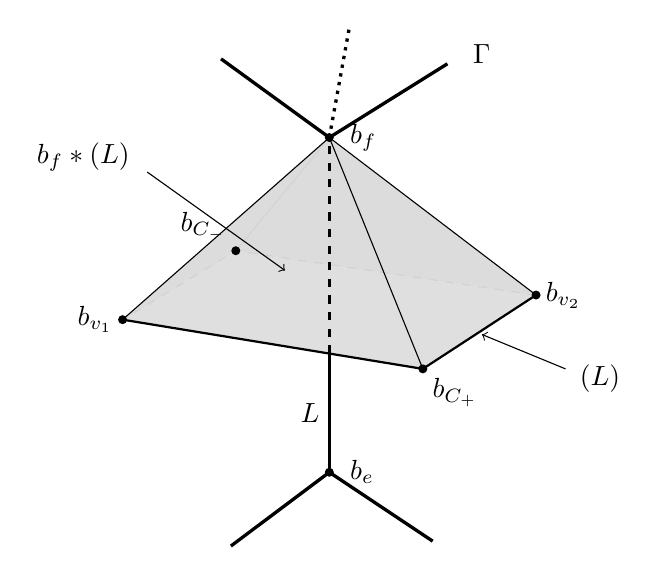
\begin{tikzpicture}[scale=1.25,line join=round]
\coordinate (be) at (0,-0.2);
\coordinate (bf) at (0,3.2);
\coordinate (v1) at (-2.1,1.35);
\coordinate (Cp) at (0.95,0.85);
\coordinate (v2) at (2.1,1.6);
\coordinate (Cm) at (-0.95,2.05);
\coordinate (cross) at (0,1.006);
\fill[gray!12] (bf) -- (v2) -- (Cm) -- cycle;
\fill[gray!12] (bf) -- (Cm) -- (v1) -- cycle;
\draw[gray!60] (bf) -- (Cm);
\draw[gray!70,dashed] (v2) -- (Cm) -- (v1);
\fill[gray!30,opacity=0.85] (bf) -- (v1) -- (Cp) -- cycle;
\fill[gray!30,opacity=0.85] (bf) -- (Cp) -- (v2) -- cycle;
\draw (bf) -- (v1); \draw (bf) -- (Cp); \draw (bf) -- (v2);
\draw[thick] (v1) -- (Cp) -- (v2);
\draw[very thick] (be) -- (cross);
\draw[very thick,dashed] (cross) -- (bf);
\draw[very thick] (bf) -- (-1.1,4.0);
\draw[very thick] (bf) -- (1.2,3.95);
\draw[very thick,dotted] (bf) -- (0.2,4.3);
\draw[very thick] (be) -- (-1.0,-0.95);
\draw[very thick] (be) -- (1.05,-0.9);
\foreach \p in {be,bf,v1,v2,Cp,Cm} \fill (\p) circle (1.3pt);
\node[right=4pt] at (be) {$b_e$};
\node[right=4pt] at (bf) {$b_f$};
\node[left] at (v1) {$b_{v_1}$};
\node[right] at (v2) {$b_{v_2}$};
\node[below right] at (Cp) {$b_{C_+}$};
\node[above left] at (Cm) {$b_{C_-}$};
\node[left] at (0,0.4) {$L$};
\node at (2.75,0.75) {$\cyLk(L)$};
\draw[->,thin] (2.4,0.85) -- (1.55,1.2);
\node at (-2.5,3.0) {$b_f*\cyLk(L)$};
\draw[->,thin] (-1.85,2.85) -- (-0.45,1.85);
\node at (1.55,4.05) {$\Gamma$};
\end{tikzpicture}
\caption{A leg $L=[b_e,b_f]$ of $\Gamma$, its link $\cyLk(L)$ in $\mathfrak K_0$, and the cone $b_f*\cyLk(L)$. The link passes
alternately through the vertex regions of the lower rays of the end points of $e$ and the open facets of the two maximal
cells containing $f$; with a coefficient $X\in\cyInv(A)$ its itinerary is the meridian class $\pm m_A(X)$. The cone meets
$\Gamma$ only at its apex $b_f$, where $X$ is a flat section.}\label{fig:meridian}
\end{figure}

\begin{lemma}[the complement lemma]\label{lem:complement}
$\ker\deg=I_\Gamma$.
\end{lemma}

The lemma says that every degree-zero class in the complement is generated by meridians with invariant coefficients.
The constant-coefficient assertion follows from $H_1(B;\Z)=0$. For the local system, the additional obstruction is
measured by the quotient of $N$ by the invariant lattices. Its two-cycles split into cochains on the graphs
$\Gamma\cap\partial F_u$. Since each $\partial F_u$ is a two-sphere, these cochains come from vertex functions.
Unimodularity then lifts the vertex functions to vectors in $N$ over the integers. These are the two steps of the proof
below; the last step is what excludes a finite-index obstruction.

\begin{proof}
Let $X_0$ be the two-dimensional cell complex obtained from the graph $G_0$ by attaching one square $\square_A$ for each arc
$A=C([u,u'],[n,n'])$ along the edge loop $(u,n),(u',n),(u',n'),(u,n')$. On $X_0$ consider the coefficient system $\hat\Lambda$
of subgroups of $N$ given by $u^\perp\cap N$ at the vertex $u$ and on the edges $(u,n)$, by $N$ at the vertex $n$, and by
$[u,u']^\perp\cap N$ on $\square_A$, with inclusions as restriction maps. Then $C_*(X_0;\hat\Lambda)$ is a subcomplex of
$C_*(X_0)\otimes N$. Its $1$-cycles are the $x$ with $\sum_nx_{un}=0$ and $\sum_ux_{un}=0$ in $N$, which is $\ker\deg$ because
$n\ne0$; and with suitable orientations of the squares $\partial(X\cdot \square_A)=m_A(X)$, so its $1$-boundaries form $I_\Gamma$. The
claim is $H_1(X_0;\hat\Lambda)=0$. Let $\mathcal Q=N/\hat\Lambda$. It is $0$ at the vertices $n$; $N/(u^\perp\cap N)\cong\Z$ by
$\langle u,\cdot\rangle$ at $u$ and on the edges $(u,n)$; and $N/([u,u']^\perp\cap N)\cong\Z^2$ by $(\langle u,\cdot\rangle,
\langle u',\cdot\rangle)$ on $\square_A$, these maps being onto because $u$, $u'$ are part of a basis of $M$
(Lemma~\ref{lem:stalks}(3)). The exact sequence of $0\to\hat\Lambda\to N\to\mathcal Q\to0$ contains
\[
H_2(X_0;N)\to H_2(X_0;\mathcal Q)\to H_1(X_0;\hat\Lambda)\to H_1(X_0;N),
\]
and we show that the last group vanishes and the first map is onto.

(a) $H_1(X_0;N)=H_1(X_0;\Z)\otimes N$ since $N$ is free, and $H_1(X_0;\Z)$ is the quotient of $H_1(G_0;\Z)$ by the classes of
the attaching loops. Lemma~\ref{lem:nerve}, with $\Lambda$ replaced by the constant system $\Z$, identifies
$H_1(B\setminus\Gamma;\Z)$ with $H_1(G_0;\Z)$, and carries the class of $\cyLk(L)$, $L\subset A$, to $\pm$ the attaching loop of
$\square_A$. So it suffices that the meridians $\cyLk(L)$ generate $H_1(B\setminus\Gamma;\Z)$. Let $U\supset\Gamma$ be the
neighbourhood of Section~\ref{ssec:normal} for $\mathfrak K=\mathfrak K_0$, and $\mathfrak E$ the union of the simplices of
$\mathfrak K_0'$ disjoint from $\Gamma$; then $B=U\cup \mathfrak E$, $U\cap \mathfrak E=\partial U$, and $B\setminus\Gamma$ retracts onto $\mathfrak E$ as
above. In the Mayer--Vietoris sequence $H_1(\partial U)\to H_1(U)\oplus H_1(\mathfrak E)\to H_1(B)=0$, a class $(0,\gamma)$ is the image
of a class of $H_1(\partial U)$ that vanishes in $H_1(U)$, that is, of a boundary $\partial\vartheta$, $\vartheta\in H_2(U,\partial U;\Z)$.
By Lemma~\ref{lem:nbhd}(3), $\vartheta$ is a sum of discs $\bar D(L)$, $L$ a leg, so $H_1(\mathfrak E)$ is generated by the circles
$\partial\bar D(L)$. The closed star $L*\cyLk(L)$ of $L$ in $\mathfrak K_0$ meets $\Gamma$ only in $L$, because $\Gamma$ is full,
and the radial projection along the join lines is a deformation retraction of $(L*\cyLk(L))\setminus L$ onto $\cyLk(L)$. It maps
$\partial\bar D(L)$, which lies in $(L*\cyLk(L))\setminus L$, homeomorphically onto $\cyLk(L)$: it sends the barycentre of $L*s$ to
the barycentre of $s$, and the segment between two such barycentres onto a segment. Hence $[\partial\bar D(L)]=\pm[\cyLk(L)]$ in
$H_1(B\setminus\Gamma)$.

(b) There are no three-cells, so $H_2(X_0;\mathcal Q)$ is the group of $2$-cycles. A $2$-chain with coefficients in $\mathcal Q$ is a
family of integers $p=(p^{(u)}_A)$, one for each arc $A$ and each vertex $u$ of $\tau_A$, where $A=C(\tau_A,\omega_A)$; the
boundary of $C_*(X_0;\mathcal Q)$ in degree two decouples over $u$, the component on the edge $(u,n)$ involving only the
$p^{(u)}$. Fix $u$ and let $S_u=\partial F_u$, a two-sphere oriented as the boundary of $F_u$. By (D2), $S_u$ is the union
of the cells $C(\tau,\omega)$ with $u\in\tau$ and $\dim\tau\ge1$, a subcomplex of the dual-pair complex. Its cells in $\Gamma$
form the graph $\Gamma_u=\Gamma\cap S_u$, whose one-cells are the arcs $A$ with $u\in\tau_A$; its other cells are the
$C(\tau,n)$, which group, according to $n$, into the sets $D^u_n=S_u\cap\widetilde R_n$. Each nonempty $D^u_n$ is connected:
its cells are the $C(u*\sigma,n)$, $\sigma$ a simplex of the link of $u$ in the triangulation of the face $n^\vee$ of
$\Delta^\circ$, with $C(u*\sigma,n)$ in the closure of $C(u*\sigma',n)$ when $\sigma\supseteq\sigma'$. That link is
connected: $n^\vee$ is a facet of $\Delta^\circ$ if $n$ is a vertex of $\Delta$, an edge of lattice length one (with $u$ an end
point) if $n$ is the centre of a pentagon or hexagon, and a point if $n$ lies in the interior of a facet of $\Delta$, and the
link of a vertex in a triangulated three-polytope is a disc or a sphere. So the $D^u_n$ are the components of
$S_u\setminus\Gamma_u$. An arc
$A=C([u,u'],[n,n'])$ lies in the closure of exactly two two-cells of $S_u$, $C([u,u'],n)\subseteq D^u_n$ and
$C([u,u'],n')\subseteq D^u_{n'}$, with opposite incidences; the two-face $F_{uu'}$ is oriented oppositely as a face of
$S_u$ and of $S_{u'}$, so the orientation of $\square_A$ can be chosen so that, for both $u$ and $u'$, the coefficient of
$\partial(p\,\square_A)$ on $(u,n)$ is $p$ times the incidence of $C([u,u'],n)$ with $A$ in $S_u$. With this choice, $p$ is a cycle
if and only if, for every $u$ and $n$, the $1$-cochain $p^{(u)}$ on the arcs of $\Gamma_u$ satisfies
\[
\sum_{\text{two-cells }f\subseteq D^u_n}\bigl(\delta\tilde p^{(u)}\bigr)(f)=0,
\]
where $\tilde p^{(u)}$ extends $p^{(u)}$ by zero to the one-cells of $S_u$ not in $\Gamma_u$ and $\delta$ is the cellular
coboundary of $S_u$.

Consider the exact sequence $0=H^1(S_u)\to H^1(\Gamma_u)\to H^2(S_u,\Gamma_u)$. The relative cellular cochains of
$(S_u,\Gamma_u)$ split as $\bigoplus_nC^*_n$, the cochains on the cells of $D^u_n$, since the coboundary of a cell $C(\tau,n)$
consists of cells $C(\tau',n)$. Each one-cell of $D^u_n$ lies on exactly two two-cells, both in $D^u_n$, with opposite
incidences, and $D^u_n$ is connected, so the sum of the values on the two-cells identifies $C^2_n/\delta C^1_n$ with $\Z$;
thus $H^2(S_u,\Gamma_u)=\bigoplus_n\Z$, and the connecting map sends the class of $p^{(u)}$ to the family of sums displayed
above. Therefore the $u$-components of $2$-cycles are exactly the coboundaries $p^{(u)}=\delta\varphi_u$ of functions
$\varphi_u$ on the vertices of $\Gamma_u$, that is, the integral combinations $\sum_v\varphi_u(v)\,\delta_u[v]$ of the vertex
cochains $\delta_u[v]$, which are $\pm1$ on the arcs of $\Gamma_u$ at $v$ and $0$ elsewhere (arcs have distinct end points).

For a $\Gamma$-vertex $v=C(\tau_v,\omega_v)$ let $\Sigma_v$ be the sum of the squares $\square_A$ of the arcs at $v$, with signs
making it a $2$-cycle of $X_0$ with integer coefficients: at a negative vertex or node the arcs are the $C(\tau_v,\varepsilon)$,
$\varepsilon$ an edge of $\omega_v$, and each edge $(u,n)$, $n$ a vertex of $\omega_v$, occurs in the two squares of the edges of
$\omega_v$ at $n$; at a positive vertex the arcs are the $C(\tau_1,\omega_v)$, $\tau_1$ an edge of $\tau_v$, and each edge
$(u,n)$ occurs in the two squares of the edges of $\tau_v$ at $u$. For $y\in N$ the image of $y\cdot\Sigma_v$ in
$C_2(X_0;\mathcal Q)$ has $u$-component, for $u\in\tau_v$, equal to $\langle u,y\rangle$ times a cycle supported on the arcs of
$\Gamma_u$ at $v$ with entries $\pm1$. The cycles supported on these arcs form a group of rank at most one. Indeed, the arcs of
$\Gamma_u$ at $v$ are the $C(\tau_1,\omega_1)$ at $v$ with $u\in\tau_1$; for such a cycle the condition attached to $D^u_n$
involves exactly the arcs at $v$ whose lower support contains $n$, each with coefficient $\pm1$; and the graph on the arcs at
$v$ in which two are joined when their lower supports share a vertex is connected (a cycle for a negative vertex or node, and
two arcs with the same lower support for a positive vertex). So the value on one arc determines the others. As $\delta_u[v]$ is such a cycle with entries $\pm1$, the $u$-component of the
image of $y\cdot\Sigma_v$ is $\epsilon_u(v)\langle u,y\rangle\,\delta_u[v]$ with $\epsilon_u(v)=\pm1$.

Now let $p$ be a $2$-cycle, $p^{(u)}=\sum_v\varphi_u(v)\,\delta_u[v]$. By Lemma~\ref{lem:stalks}(3) the map $N\to\Z^{\tau_v}$,
$y\mapsto(\langle u,y\rangle)_{u\in\tau_v}$, is onto, so there are $y_v\in N$ with $\langle u,y_v\rangle=\epsilon_u(v)\varphi_u(v)$ for
all $u\in\tau_v$. Then $\sum_vy_v\cdot\Sigma_v\in H_2(X_0;N)$ maps to $p$. So $H_2(X_0;N)\to H_2(X_0;\mathcal Q)$ is onto, and
$H_1(X_0;\hat\Lambda)=0$.
\end{proof}

\begin{theorem}[filling]\label{thm:filling}
$\partial Z(\mathfrak K_0)=\cyBal$.
\end{theorem}

\begin{proof}
$\partial Z(\mathfrak K_0)\subseteq\cyBal$ because $\partial\partial=0$. Let $\beta\in\cyBal$ and let $\zeta$, $b$, $\theta$, $b'$ be as in
Steps~1 and~2. By Lemmas~\ref{lem:nerve} and~\ref{lem:complement}, $\cyit[b']\in\ker\deg=I_\Gamma$, so
$\cyit[b']=\sum_i m_{A_i}(X_i)$ for finitely many arcs $A_i$ and $X_i\in\cyInv(A_i)$. Choose a leg $L_i\subset A_i$ with
apex $b_{f_i}$, and signs so that $\cyit[X_i\cdot\cyLk(L_i)]=m_{A_i}(X_i)$. Then $b'-\sum_iX_i\cdot\cyLk(L_i)$ is a $1$-cycle on
$\mathfrak K_0^\circ$ with itinerary zero, hence null-homologous in $B\setminus\Gamma$ (Lemma~\ref{lem:nerve}), hence the boundary
$\partial y_0$ of a $2$-chain $y_0$ on $\mathfrak K_0^\circ$ with coefficients in $\Lambda$. Put
\[
z:=\zeta-\theta+y_0+\sum_iX_i\cdot\bigl(b_{f_i}*\cyLk(L_i)\bigr)\in C_2(\mathfrak K_0;F).
\]
Since $\beta=b+\partial\zeta$, $b=b'-\partial \theta$, $b'=\partial y_0+\sum_iX_i\cdot\cyLk(L_i)$ and $\partial(b_f*c)=c$ for a $1$-cycle
$c$, we get $\partial z=\beta$. So $z\in Z(\mathfrak K_0)$ with boundary network $\beta$.
\end{proof}

\begin{proof}[Proof of Theorem~\ref{thm:real}]
By Theorem~\ref{thm:filling} and Proposition~\ref{prop:rhoH},
\[
\rho(Z(\mathfrak K_0))=\rho(\partial Z(\mathfrak K_0))=\rho(\cyBal)=K.
\]
For any triangulation $\mathfrak K$ of $B$ in which $\Gamma$ is full, $\partial Z(\mathfrak K)\subseteq\cyBal$
(Section~\ref{ssec:coef}), so $\rho(Z(\mathfrak K))\subseteq K$.
\end{proof}

If $\mathfrak K$ is a subdivision of $\mathfrak K_0$ in which $\Gamma$ is full, the subdivision operator carries $Z(\mathfrak K_0)$
into $Z(\mathfrak K)$ without changing node coefficients, so $\rho(Z(\mathfrak K))=K$ as well.

\begin{remark}[no torsion]\label{rem:notorsion}
Every step is integral: $H_1(D_\varepsilon,\partial D_\varepsilon)=0$, $H_1(\mathcal X)=0$, $H^1(S^2)=0$, $H_1(S^3)=0$, and the
unimodularity of $\mathcal T$ in Lemma~\ref{lem:stalks}(3). No condition on the torsion of $H_2(\widehat X;\Z)$ or of
$H_1(B;\iota_*\Lambda)$ enters, and $\rho(Z(\mathfrak K_0))$ is $K$ itself, not a sublattice of finite index.
\end{remark}

\begin{remark}[where $K$ enters]\label{rem:whereK}
The lattice $K$ enters only through Proposition~\ref{prop:rhoH}. Theorem~\ref{thm:filling} holds for every balanced network,
whatever its node coefficients, and its proof uses Hypothesis~\ref{hyp:P} only through the existence of $B$, admissibility
through the list of $\Gamma$-vertices (D3), and Theorem~\ref{thm:U} through Lemma~\ref{lem:stalks}(2),(3). The fillings it
constructs consist of sheets $\zeta_\varepsilon\otimes d_\varepsilon$ in the dual discs, with coefficients in $\Z d_\varepsilon$ and
containing arcs and positive vertices in their interior; pairs of triangles at the $\Gamma$-points of the dual paths, with
coefficients in $\cylin(\omega)$; cones $b_f*\cyLk(L)$ crossing a leg at $b_f$ with an invariant coefficient; and a
$\Lambda$-valued $2$-chain in $B\setminus\Gamma$. The finite computations illustrating the theorem are described in Section~\ref{ssec:list}.
\end{remark}
